\chapter{Admin podstránka}

keďže stránka bola tvorená pre klienta bez znalostí programovania v prostredí php a MySQL, tým pádom musí byť nastavovanie všetkých parametrov stránok veľmi intuitívne a najlepšie tvorené pomocou formulárov s nápismi čo treba robiť a kam pridať aké formáty súborov. Z toho dôvodu je vytvorené programátorské prostredie, ktoré je ale zabezpečené pred nechceným vstupom menom a heslom. Na utvorenie funkcie prihlasovania boli použité časti kódu, z open-source návodu \cite{login}. Pre vstup do login.php môžeme tento link napísať priamo do vyhľadávača, alebo do tejto stránky vstúpime pomocou skrytého tlačidla schovaného v pravom dolnom rohu stránky index.php.

\section{Prístup do prostredia admin}

Ako už bolo spomenuté, do programátorského prostredia vstupujeme pomocou tlačidla/linku presmerovaného na podstránku login.php obr.\ref{OBRAZOK 1.8}. Pokiaľ sa už užívateľ raz do konta prihlásil, zostane prihlásený a teda nemusí sa vždy znova prihlasovať. Programátorské prostredie je designovo veľmi jednoduché obr.\ref{OBRAZOK 1.9}, podstatná je funkcionalita všetkých jeho podstránok a to menovite:

\begin{itemize}
\item upload image: pridávanie fotiek do podstránky foto.php
\item add post: pridávanie článkov do podstránky indexx.php
\item manage post: úprava článkov podstránky indexx.php
\item reset your password: reset hesla
\item sign out of your account: odhlasit sa z \verb|hVe@7hL[8mk'x}=.php|
\item register new account: registrácia nového admina
\item home: presmerovanie na index.php
\end{itemize}

Pre potreby zabezpečenia programátorského prostredia je jeho názov komplikovaný a to síce \verb|hVe@7hL[8mk'x}=.php|, je to z dôvodu aby užívateľ náhodne nenapísal do prehliadača admin.php alebo podobné logické názvy stránok, ktoré by úplne preskočili zabezpečenie pomocou login.php.

\pagebreak

\begin{figure}[!tbh]
\centering
\setlength{\fboxsep}{0pt}%
\setlength{\fboxrule}{1pt}%
\fbox{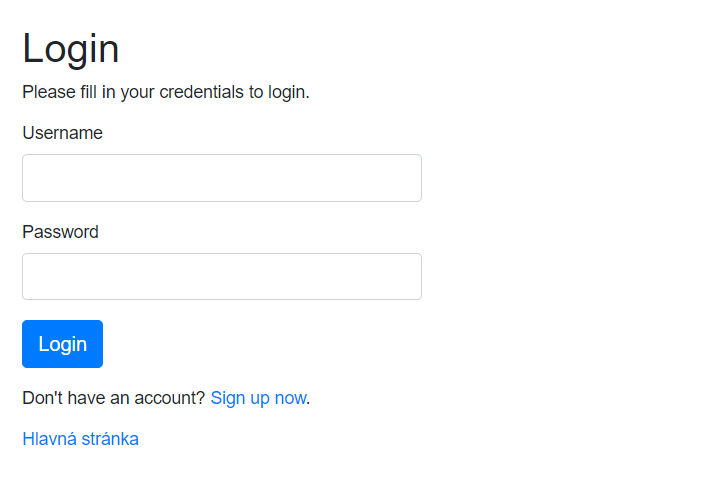
\includegraphics[width=\textwidth]{obr/login_page.png}}
\caption{Prihlasovanie do programátorského prostredia pomocou login.php.}\label{OBRAZOK 1.8}
\end{figure}

\begin{figure}[!tbh]
\centering
\setlength{\fboxsep}{0pt}%
\setlength{\fboxrule}{1pt}%
\fbox{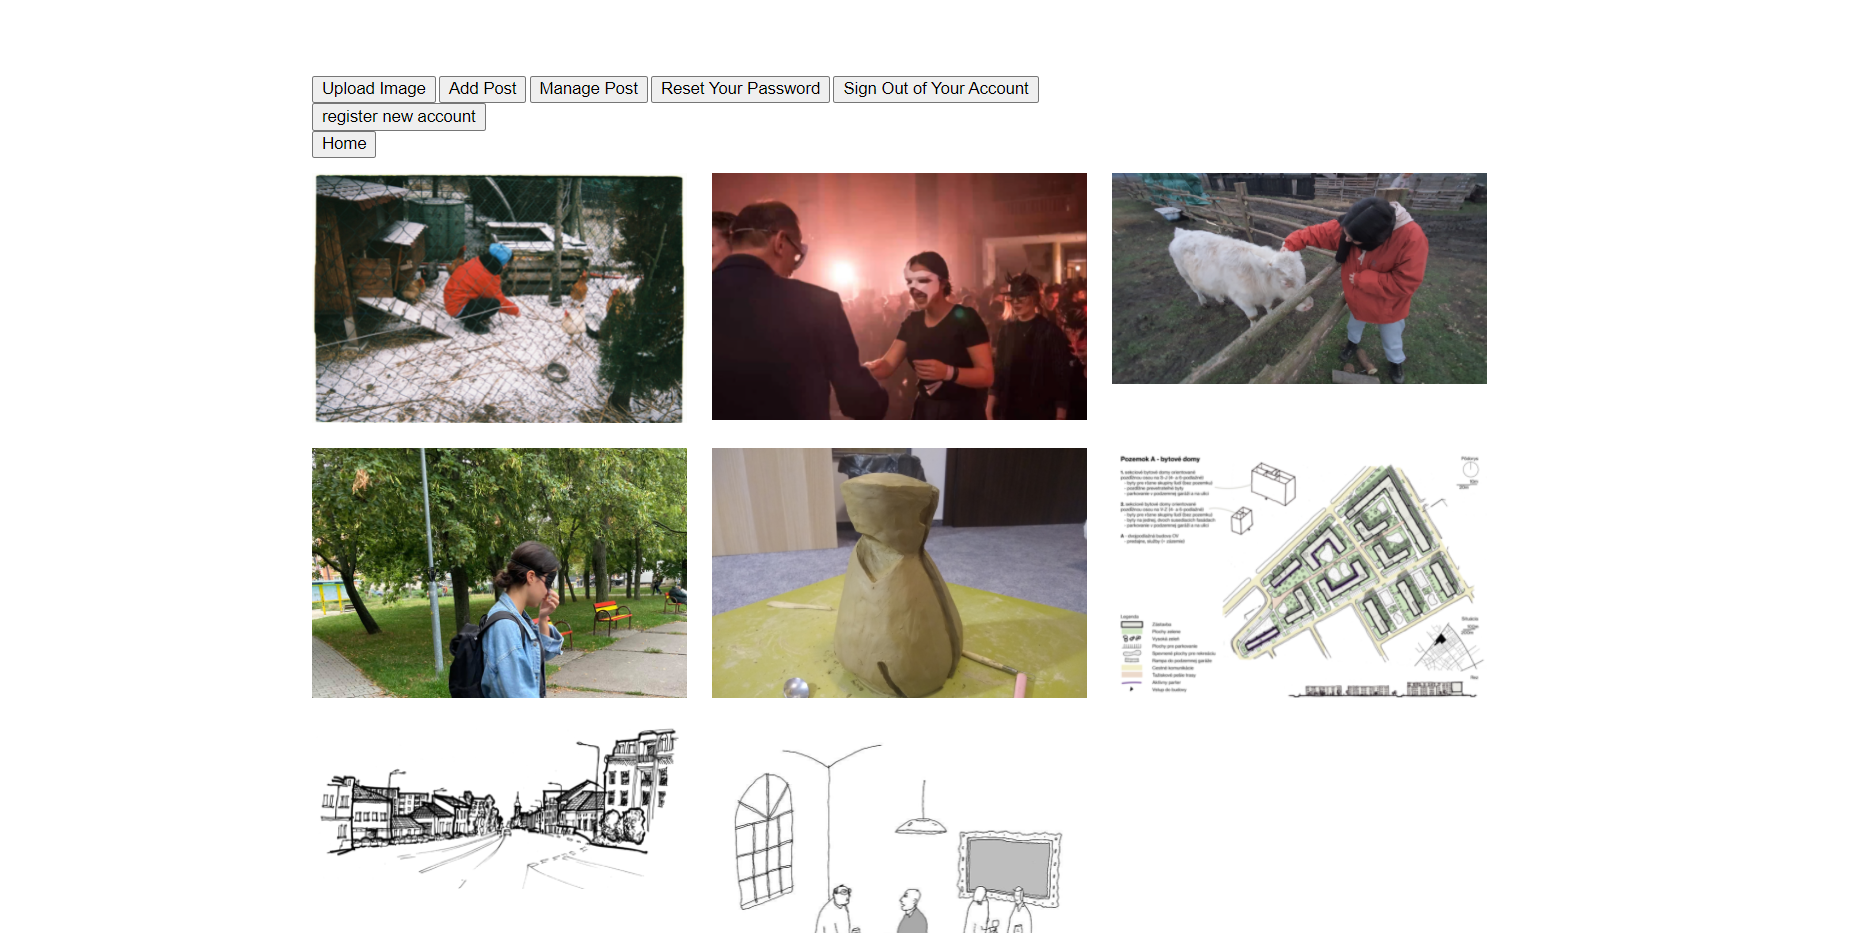
\includegraphics[width=\textwidth]{obr/admin.png}}
\caption{Programátorské prostredie}\label{OBRAZOK 1.9}
\end{figure}

\pagebreak

\section{Tlačidlá v prostredí admin}
\subsection{upload image}

Tlačidlo Upload image, nás presmeruje na podstránku upload.php obr.\ref{OBRAZOK 1.10} kde sa pomocou formuláru pridávajú fotky na podstránku foto.php. Ku fotke pridávame nadpis, popis a samotnú fotku.

\begin{figure}[!tbh]
\centering
\setlength{\fboxsep}{0pt}%
\setlength{\fboxrule}{1pt}%
\fbox{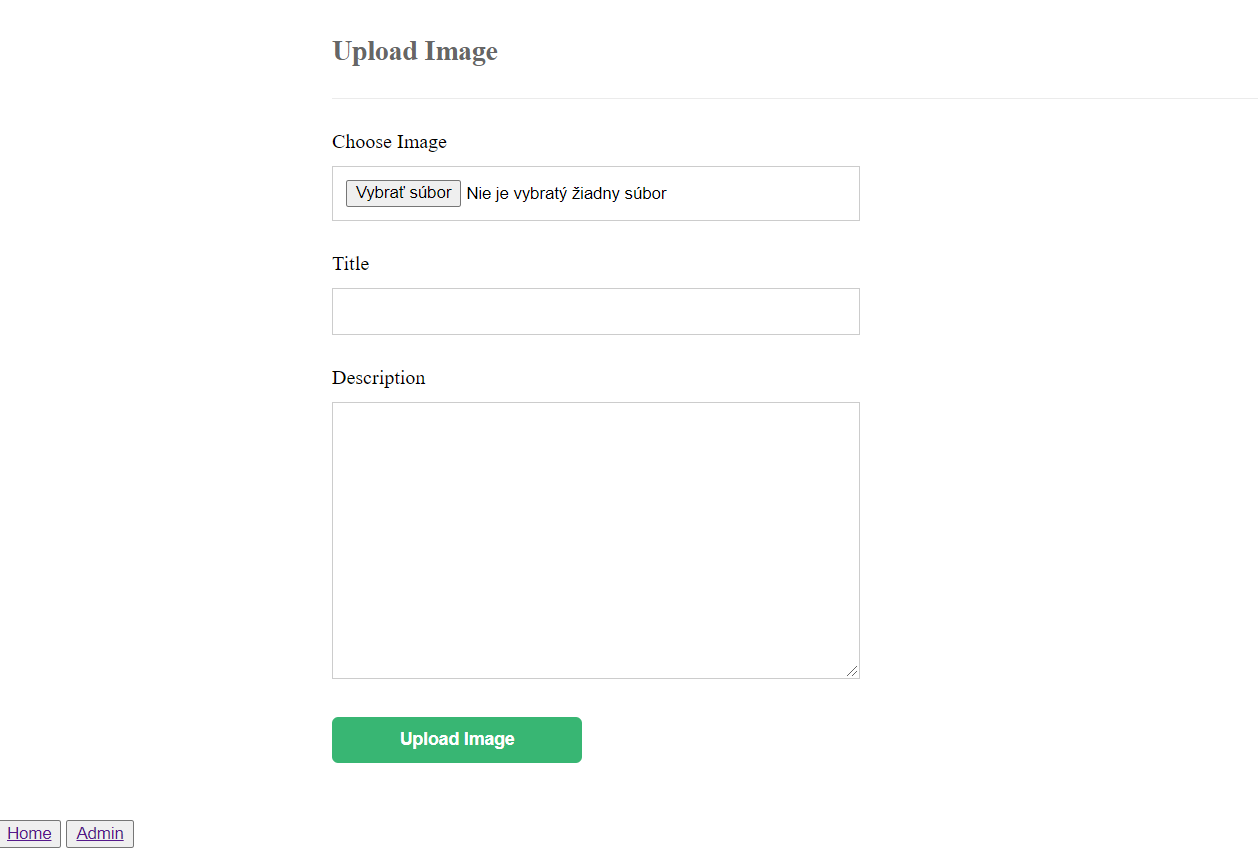
\includegraphics[width=8cm]{obr/upload_image.png}}
\caption{Upload image, podstránka upload.php }\label{OBRAZOK 1.10}
\end{figure}

\subsection{add post}

Tlačidlo add post, nás presmeruje na podstránku \verb|add_post.php| obr.\ref{OBRAZOK 1.11} kde sa pomocou formuláru pridávajú články na podstránku indexx.php. Ku článku pridávame jeho názov, obsah a voliteľnou položkou je kategória(možná implementácia, momentálne nepoužívaná funkcia).

\begin{figure}[!tbh]
\centering
\setlength{\fboxsep}{0pt}%
\setlength{\fboxrule}{1pt}%
\fbox{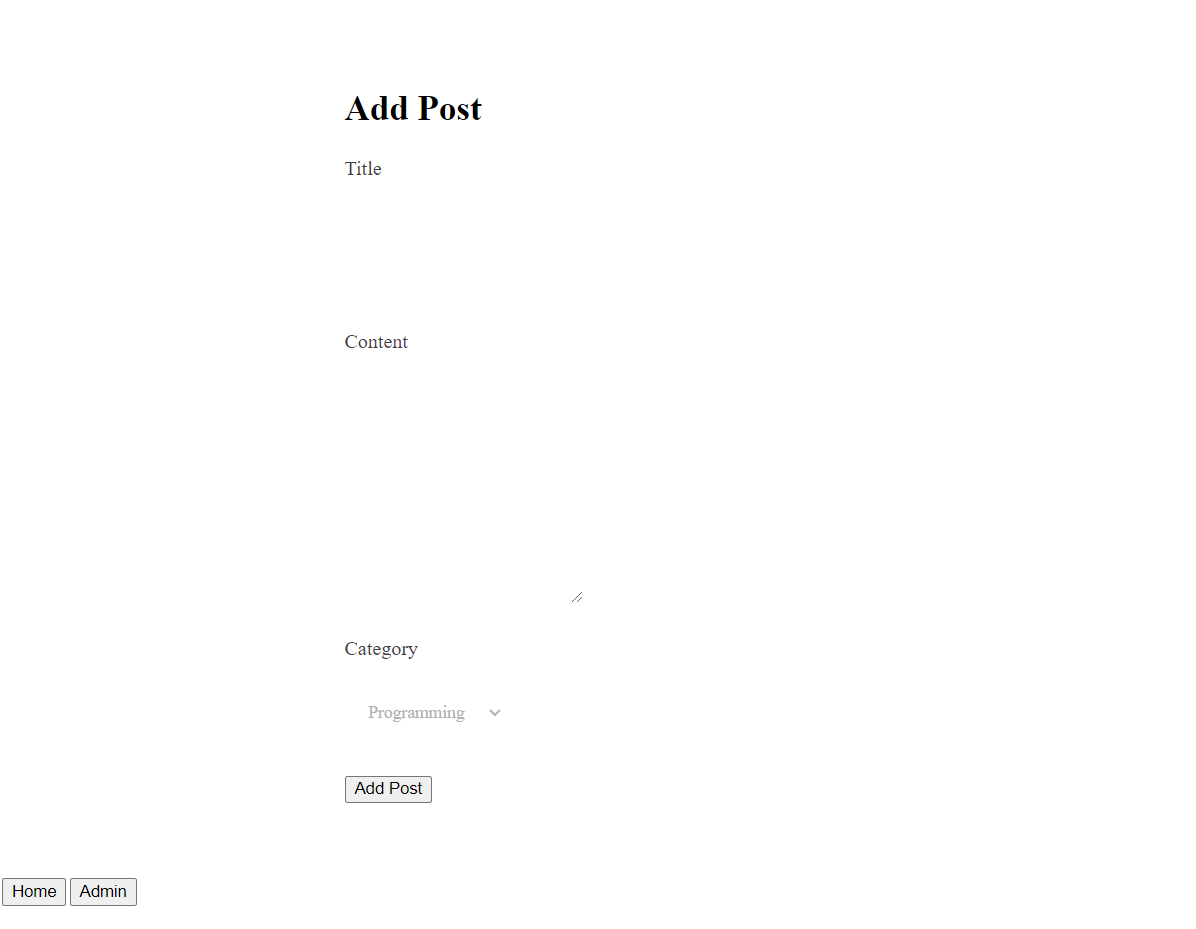
\includegraphics[width=8cm]{obr/addpost.png}}
\caption{add post, podstránka addpost.php}\label{OBRAZOK 1.11}
\end{figure}

\subsection{manage post}

Tlačidlo manage post, nás presmeruje na podstránku \verb|manage_posts.php| obr.\ref{OBRAZOK 1.12} kde sa pomocou formuláru a tlačidiel upravujú články na podstránku indexx.php.

\begin{figure}[!tbh]
\centering
\setlength{\fboxsep}{0pt}%
\setlength{\fboxrule}{1pt}%
\fbox{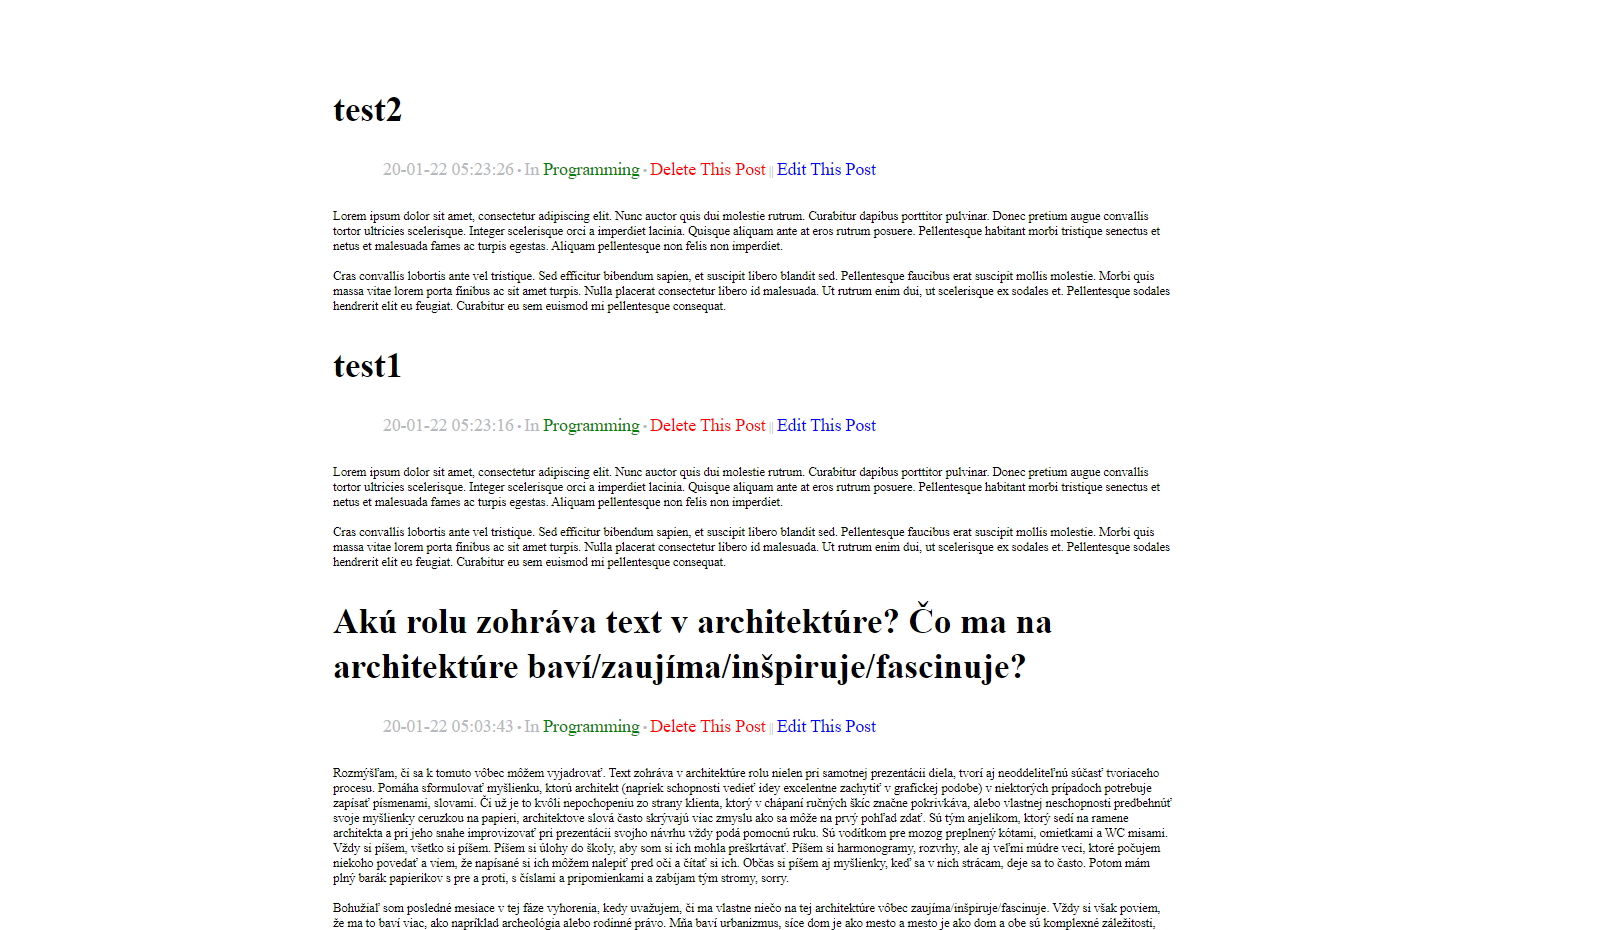
\includegraphics[width=8cm]{obr/manageposts.png}}
\caption{manage post, podstránka manageposts.php}\label{OBRAZOK 1.12}
\end{figure}

\subsection{reset your password}

Tlačidlo reset your password, nás presmeruje na podstránku \verb|reset-password.php| obr.\ref{OBRAZOK 1.13} kde sa pomocou formuláru mení heslo potrebné na prístup do programátorského prostredia.

\begin{figure}[!tbh]
\centering
\setlength{\fboxsep}{0pt}%
\setlength{\fboxrule}{1pt}%
\fbox{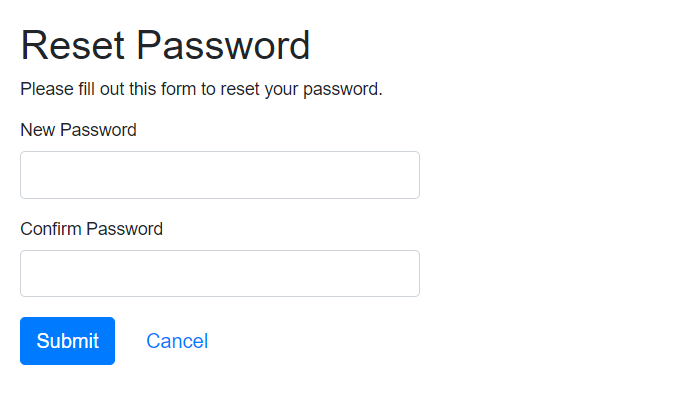
\includegraphics[width=8cm]{obr/resetpass.png}}
\caption{reset your password, podstránka reset-password.php}\label{OBRAZOK 1.13}
\end{figure}

\subsection{sign out of your account}

Tlačidlo sign out of your account, nás odhlási z účtu ktorým je administrátor prihlásený do programátorského prostredia.

\pagebreak

\subsection{register new account}

Tlačidlo register new account, nás presmeruje na podstránku \verb|registerreal.php| obr.\ref{OBRAZOK 1.14} kde sa pomocou formuláru pridávajú nový administrátori pre vstup do programátorského prostredia.

\begin{figure}[!tbh]
\centering
\setlength{\fboxsep}{0pt}%
\setlength{\fboxrule}{1pt}%
\fbox{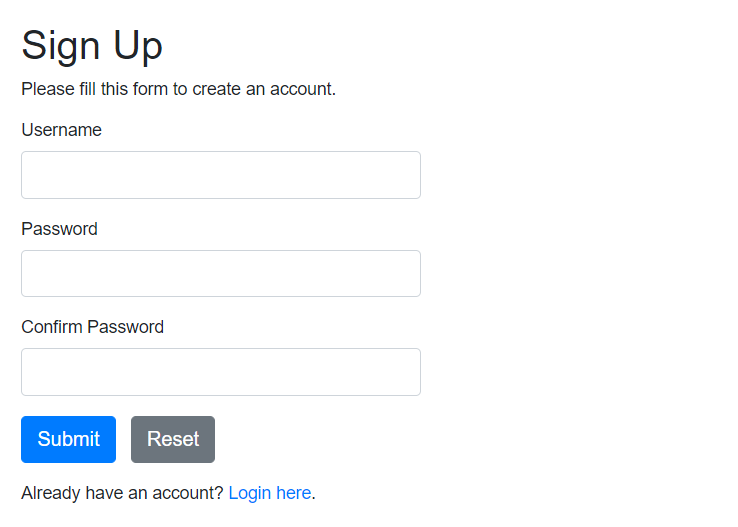
\includegraphics[width=8cm]{obr/signup.png}}
\caption{register new account, podstránka registerreal.php}\label{OBRAZOK 1.14}
\end{figure}

\subsection{home}

Tlačidlo home, nás presmeruje na úvodnú stránku, index.php.

\subsection{vymazávanie fotiek}

Vymazávanie fotiek funguje na princípe načítania všetkých fotiek v programátorskom prostredí a ich zobrazenie ako na podstránke foto.php. Avšak pri fotke nám pribudlo červené tlačidlo obr.\ref{OBRAZOK 1.15} ktoré užívateľa presmeruje na podstránku delete.php kde je vykonané druhotné potvrdenie vymazania fotky, aby nedochádzalo k ich náhodnému a nechcenému vymazávaniu.

\begin{figure}[!tbh]
\centering
\setlength{\fboxsep}{0pt}%
\setlength{\fboxrule}{1pt}%
\fbox{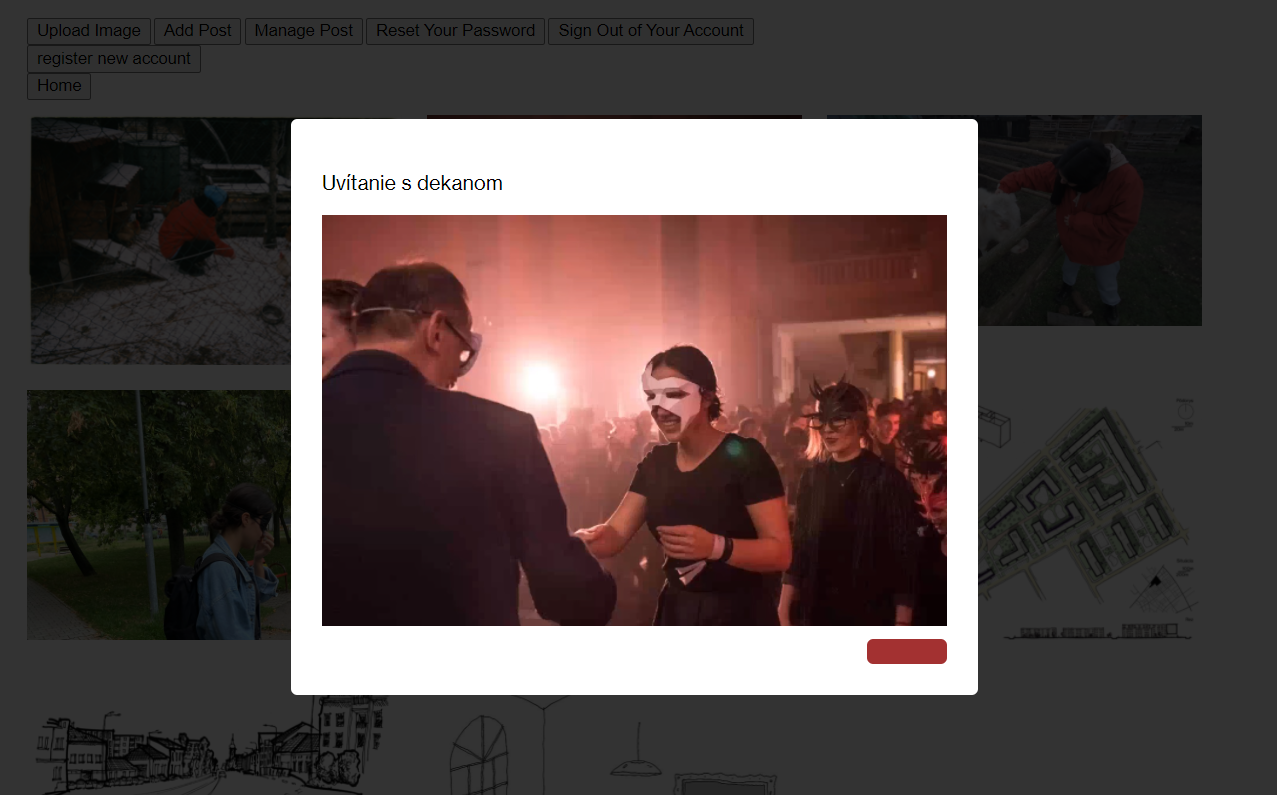
\includegraphics[width=8cm]{obr/adminvymazaniefoto.png}}
\caption{vymazávanie fotiek v programátorskom prostredí}\label{OBRAZOK 1.15}
\end{figure} 